\documentclass[12pt,a4paper]{book}
\usepackage[english]{babel}
\usepackage[latin1]{inputenc}
\usepackage{times}
\usepackage{url}
\usepackage{graphicx}
\usepackage{subfigure}
\usepackage{makeidx}
\usepackage{tocbibind}
\usepackage[pagebackref,plainpages=false]{hyperref}

\newenvironment{comment}{\footnotesize \begin{quote}}{\end{quote}}

\newenvironment{code}
	       {\begin{quote}}
	       {\end{quote}}
\newcommand{\keyword}[1]{\texttt{#1}}
\newcommand{\function}[1]{\texttt{#1}}
\newcommand{\variable}[1]{\emph{#1}}
\newcommand{\constant}[1]{\texttt{#1}}
\newcommand{\errno}[1]{\texttt{#1}}


\title{Viengoos Developer Reference}
\author{Neal H. Walfield}
\date{January 2008}

\begin{document}

\frontmatter
\maketitle
\tableofcontents

\mainmatter

\setlength{\parindent}{0pt}
\setlength{\parskip}{1ex plus 0.5ex minus 0.2ex}

\chapter{Introduction}

Viengoos is an extensibility, object-capability system, ala Hydra
\cite{wulf74hydra} and EROS \cite{shapiro99eros}.  

Viengoos was built on the following ideas:

\begin{itemize}
\item object based,
\item no kernel dynamic allocation,
\item resource accountability,
\item atomic methods,
\item object statelessness \cite{tullmann96userlevel-checkpointing-through-exportable-kernel-state},
\item caching \cite{cheriton94caching-model-of-os-kernel-functionality}
\item interrupt model \cite{ford99interface-and-execution-models},
\item activation-based \cite{roscoe95structure-of-a-multi-service-os}, and
\item resilience to destructive interference \cite{miller06robust-composition}
\end{itemize}

This reference is divided into two parts.  The first describes the
kernel, how object addressing works, the primordial objects and
resource management mechanisms and policies.  The second part
describes the sample run-time environment shipped with Viengoos.

\part{Viengoos}

\chapter{Addressing}

\begin{quotation}
  ``The name of the song is called `HADDOCKS' EYES.'\,''

  ``Oh, that's the name of the song, is it?'' Alice said, trying to feel
  interested.

  ``No, you don't understand,'' the Knight said, looking a little vexed.
  ``That's what the name is CALLED.  The name really IS `THE AGED AGED
  MAN.'\,''

  ``Then I ought to have said `That's what the SONG is called'?''
  Alice corrected herself.

  ``No, you oughtn't: that's quite another thing!  The SONG is called
  `WAYS AND MEANS': but that's only what it's CALLED, you know!''

  ``Well, what IS the song, then?'' said Alice, who was by this
  time completely bewildered.

  ``I was coming to that,'' the Knight said.  ``The song really IS
  `A-SITTING ON A GATE':  and the tune's my own invention.''

  \begin{flushright}
    \emph{Through the Looking Glass}\\
    Lewis Carroll
  \end{flushright}
\end{quotation}


Viengoos is an object-capability system.  Objects are designated
exclusively by way of capabilities.  A capability is a
kernel-protected, unforgeable reference.  Capabilities are addressed
in the context of an address space.  Each thread object has a
capability slot that represents the root of its address space.  When
the thread generates an address, the address is resolved in the
context of its address space.

This chapter first describes how capabilities work, their format, and
the kernel supported methods for manipulating capabilities.  We then
discuss addressing.  Namely, how addresses are encoded, address spaces
construction, and address resolution.

\section{Capabilities}

A capability both \emph{designates} an object and \emph{authorizes}
access to it.  (The importance of this is best illustrated with the
Confused Deputy problem \cite{hardy88confused-deputy}.)  Capabilities
are unforgeable in that they are kernel protected--their bit
representation is never exposed--and thus can only be transferred via
authorized channels.

To sense or modify an object, a capability designating it is
\emph{invoked}.  Invocation causes a message to be sent to the object.
The exact semantics of an invocation depend on the object's
implementation.

A capability may be delegated by transferring it in an object
invocation.  When a capability is transferred in such a way, the
capability is copied to the receipient's message buffer.  Because the
receive buffer is allocated beforehand, copying does not require that
the kernel allocate memory.

In Viengoos, the only way to revoke access to an object is to destroy
the object.\footnote{Revocation can be implemented by way of Redell's
  Caretaker but so far, this mechanism has not been required.}  By
destroying the object, all capabilities designating it become invalid
and act as if they designated the VOID object.

Viengoos allows user-object implementations.  A user-object is
implemented by a process.  The process allocates an end point and
distributes it to clients.  Clients may invoke the end point.  The
server process may collect the messages from the end point and act on
them as it sees fit.

As user objects are accessed in the same way as kernel objects, it is
possible to interpose on specific objects or to fully or partially
emulate the kernel from a user-space process.

\subsection{Format}

A capability is 128-bits wide and consists of the following fields:

\begin{itemize}
\item an object identifier (OID),
\item a version,
\item a weak predicate (W),
\item address translation directives,
  \begin{itemize}
  \item a guard, and
  \item a sub-page descriptor
  \end{itemize}
\item an object memory policy,
  \begin{itemize}
  \item a discardability predicate (D), and
  \item a priority
  \end{itemize}
\end{itemize}

\subsubsection{Object Identification}

The OID field is used to locate an object.  The OID corresponds to a
block of storage on backing store.  Backing store is managed by
so-called backing store managers.  When an object is referenced and
the object is not in memory, Viengoos submits a request to page the
object in to the appropriate backing store manager.  Similarly, when
Viengoos decides that the object should be flushed to persistent
store, it sends a request to the backing store manager.

When an object is destroyed, all references to it must be invalidated.
Invalidating references is difficult as it requires finding all of the
references.  Maintaining a linked list of capabilities referencing an
object requires two additional pointers per capability.  But this only
suffices for in-memory objects: if a cappage is paged-out and the
object is destroyed, these must be invalidated as well.  To work
around this problem, each object also has a version number.  When a
capability to an object is created, the object's version number is
copied into the capability.  Then, when dereferencing a capability,
the capability is only considered valid if the the version numbers
match.  If they do not match, then the reference is known to not be
valid and the VOID object is returned instead of the object instance.

The use of the version field raises another problem: it is limited in
size.  To avoid overflowing it and having to do a disk scavenge before
being able to reuse the storage, it is imperative to control its
growth.  The solution EROS has used is to only bump the field if a
capability designating the object goes to disk, a relatively rare
occurrence, they observe, and to rate-limit that to once every few
minutes \cite{citation-needed}.

\subsubsection{Weak Capabilities}

The data, cappage, endpoint, and activity objects implement two
interfaces (facets): a so-called strong facet and a weak facet.  The
weak facet allows access to a subset of the functionality that the
strong facet allows.

A capability designating the weak facet of a data-page provides
read-only access to the object.  The same applies for a cappage,
however, the access is transitively removed: strong capabilities
fetched via a weak capability are downgraded by the kernel to weak
reference the object's weak facet.  A capability designating the weak
facet of an end-point only allows enqueuing messages.  And, a
capability designating the weak facet of an activity does not allowing
changing the activity's policy.

\subsubsection{Address Translation}

In Viengoos, address spaces are composed through the arrangement of
cappages; cappages act as page-tables.  A thread object contains a
capability slot, which is filled with the root capability.  Some
object methods all take a capability designating the root.

Viengoos uses a guarded page table scheme
\cite{liedtke94page-table-structures-for-fine-grain-vm}.  To support
this, capabilities contain two fields: a guard and a subpage
descriptor.  The guard consists of a value and a length.  A subpage
descriptor allows the use of only part of a capability page in address
translation.  It consists of a subpage count and an offset.  The count
indicates the number of subpages in the cappage.  This value must be
between 1 and 256 inclusive and be a power of 2.  For example, a count
of 2 means to divide the cappage into two subpages, each consisting of
$256 / 2 = 128$ capabilities.  The offset is then used to select the
subpage to index.  Address translation is discussed in section
\ref{address-translation}.

\subsubsection{Object Memory Policy}

To allow principals to control memory is managed, each capability
contains two fields that describe the discardability and the priority
of the designated object.  When the object is accessed via the
capability, if the object is claimed,\footnote{Claiming is discussed
  in \ref{object-claiming}.} the policy is applied to the object.

The discardability property is a hint that Viengoos may, instead of
flushing changes to disk, simply discard a frame's content.  If a
capability has the weak predicate set, this hint is ignored.  If
content discarded, the next access to the object will raise a
discarded event.  If an activity is discarded, all objects allocated
against the activity are destroyed.

The priority property allows an activity to control the order in which
the frames, which it has claimed, are released.  If the content is
dirty and has not been marked as discardable, the content is written
to backing store.  Otherwise, the frame is made eligible for immediate
reuse.

The lower the numric value of the priority field, the lower the
frame's priority.  Frames are released in priority order.  If multiple
frames have the same priority, they are released in a random order
unless the priority is 0, in which case, the frames are released in
approximately LRU order.

\section{Local Addresses}

Capabilities are designated using local addresses.  Each thread object
contains a capability slot that is used as the root of the thread's
address space.  When the thread faults or otherwise causes an object
look, address translation starts at this capability.

\subsection{Address Encoding}

On Viengoos, all addresses are 64-bits wide.  This is true even on
32-bit platforms.  On these platforms, the address is automatically
extended.

Viengoos addresses consist of a {\bf prefix} and a {\bf depth}.  The
depth specifies the length of the prefix.  This type of addressing
allows, for example, addressing not only leaf objects but also
internal nodes.  (Hence, the intuition behind depth is how far into
the tree to search.)  The address prefix is encoded in the most
significant bits of the address.  This is followed by a bit with the
value of 1, and then $63 - depth$ (\var{idepth}), which is encoded in
unary.  The address with all zeros is the NULL address.  The NULL
address is sometimes used to denote some default action.  When
returned, it typically means failure.

\begin{center}
  \begin{bytefield}{32}
    \tiny{63}\hspace{\stretch{1}}\tiny{0}\\
    \bitsl{20}{depth}{prefix} & \bit{1} & \bitsl{11}{63 - depth}{idepth}
  \end{bytefield}
\end{center}

Observe that the value of idepth is the position of the least
significant bit that is on.

By convention, addresses are written \emph{prefix/depth}.

Viengoos automatically translates machine addresses to the above form.
The prefix is set to the machine address zero-extended to 63 bits and
the depth is set to 63.  For machines with 64-bits addresses,
addresses with the most significant bit set are illegal.

The root capability slot is identified with by the address 0/0.  Its
encoding is:

\begin{center}
  \begin{bytefield}{32}
    \tiny{63}\hspace{\stretch{1}}\tiny{0}\\
    \bit{1} & \bitsl{31}{63}{0}
  \end{bytefield}
\end{center}

The address 0x804b2c0 is encoded:

\begin{center}
  \begin{bytefield}{32}
    \tiny{63}\hspace{\stretch{1}}\tiny{0}\\
    \bitsl{31}{63}{0x804b2c0} & \bit{1}
  \end{bytefield}
\end{center}

The address of the data object that contains the above byte would be
the address rounded down to the nearest page size and with a depth of
63 - the logarithm base 2 of the page size.  If the underlying
hardware has base pages with a size of 4kb, then the address would be
0x804b000/51.


\subsection{Address Translation}
\label{address-translation}

Address translation starts at the root of the current address space
and consumes the address by checking guards and indexing cappages,
until all address bits are consumed.  More formally, the following
algorithm returns the object designated by the local address
\var{address}.

\begin{algorithmic}
\STATE $C \leftarrow \mbox{Root}$
\STATE $P \leftarrow \mathop{prefix}(\mbox{address})$
\STATE $R \leftarrow \mathop{depth}(\mbox{address})$
\LOOP
  \IF{$R < \mathop{guard\_length}(C)$}
    \RETURN failure \COMMENT{Not enough remaining bits to translate the guard}
  \ENDIF
  \IF {$\mathop{guard}(C) \neq P_{R..R-\mathop{guard\_length}(C) + 1}$}
    \RETURN failure \COMMENT{The guard does not match}
  \ENDIF

  \STATE $R = R - $guard\_length$(C)$
  \IF {$R = 0$}
    \RETURN cap\_to\_object$(C)$
  \ENDIF

  \STATE $S \leftarrow 256/\mathop{subpages}(C)$ \COMMENT{The subpage size}
  \IF {$R < log_2(S)$}
    \RETURN failure \COMMENT{Not enough remaining bits to index the cappage}
  \ENDIF

  \STATE $O \leftarrow $ cap\_to\_object$(C)$
  \IF{not $O$ or typeof $O \neq$ cappage}
    \RETURN failure \COMMENT{Type mismatch}
  \ENDIF

  \STATE $C \leftarrow
    O.\mbox{caps}\left[S/\mathop{subpages}(C)
    + P_{R..R-\log_2(S)+1}\right]$ \COMMENT{The next page table}

  \STATE $R \leftarrow R - \log_2(S)$
\ENDLOOP
\end{algorithmic}

\begin{figure}
  \begin{center}
    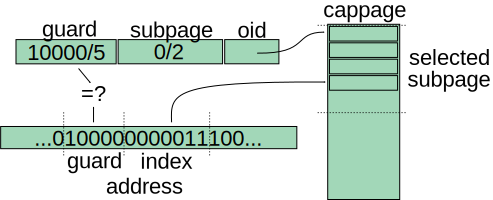
\includegraphics[width=0.9\textwidth]{gpt}
  \end{center}
  \caption[Address Translation]{Translating part of an address using a
    guarded page table entry.  First, the guard is compared.  If it
    matches, the subpage descriptor is applied to the designated
    object and the correct subpage selected.  The subpage is then
    indexed to find the next capability.  This process is repeated
    until all address bits are translated or a fault occurs.}
  \label{fig:address-translation}
\end{figure}

The translation of a guarded page table entry is illustrated in figure
\ref{fig:address-translation}.

When copying capabilities, the same principle applies, however, to
allow the easy designation of the capability that designates the
object at some address, if there are not bits remaining to translate
after translating the guard, the capability is returned.

\section{Data Structures}

\subsection{\type{addr}}

The format of an address is:

\begin{center}
  \begin{bytefield}{32}
    \tiny{63}\hspace{\stretch{1}}\tiny{0}\\
    \bit{1} & \bitsl{31}{63}{0}
  \end{bytefield}
\end{center}

\var{idepth} is stored in unary.  The depth is 63 - \var{idepth}.

\subsection{\type{addr_trans}}

The \type{addr_trans} structure has the following layout:

\begin{struct}{32}
  \bitsl{14}{22-lsp}{guard}
  & \bitsl{8}{(lsp)}{subpage}
  & \bits{4}{$log_2$ sps}
  & \bits{6}{g\_depth}
\end{struct}

\var{$log_2$ sps} is logarithm base 2 of the number of subpages.
\var{subpage} is the subpage to select.  It has a width of \var{lsp}.
\var{g\_depth} is the number of length of the guard.  \var{guard} is
the value of the guard and is zero-extended to \var{g\_depth}.  Its
width is also not fixed.

\subsection{\type{object_policy}}

The \type{object_policy} structure has the following layout:

\begin{struct}{16}
  \bits{5}{\dontcare} & \bit{D} & \bits{10}{priority}
\end{struct}

\var{D} is the discardability predicate.

\subsection{\type{cap_properties}}

The \type{cap_properties} structure has the following layout:

\begin{struct}{32}
  \bits{16}{\dontcare} & \bits{16}{object\_policy} \\
  \bits{32}{addr\_trans}
\end{struct}

\subsection{\type{cap}}

The following is the internal representation of a capability.  Only
the discardability predicate, the priority and the address translator
are exposed to the user.

\begin{struct}{32}
  \bits{20}{version} & \bit{W} & \bit{D} & \bits{10}{priority} \\
  \bits{32}{address translator} \\
  \wordbox{2}{OID}
\end{struct}

\var{D} is the discardability predicate.  \var{W} is the weak
predicate.


%%%%%%%%%%%%%%%%%%%%%%%%%%%%%%%%%%%%%%%%%%%%%%%%%%%%%%%%%%%%%%%%%%%%%
\chapter{Primordial Objects}

\begin{quotation}
\noindent
I. The world is everything that is the case.\\
I.I The world is the totality of facts, not of things.\\
I.II The world is determined by the facts, and by these being
\emph{all} the facts.\\
I.I2 For the totality of facts determines both what is the case, and
also all that is not the case.

\begin{flushright}
\emph{Tractatus Logico-Philosophicus} by Ludwig Wittgenstein
\end{flushright}
\end{quotation}

This chapter describes the primordial objects implemented by the
microkernel.  They include folios, the unit of storage allocation,
data and capability pages, threads, message buffers, end points, and
activities.  These objects represent the fundamental building blocks
of the system; all other objects are built from compositions of these
objects.

\clearpage
\section{Objects}

All objects are derived from the generic base object \type{object}.
Each object has a number (possibly zero) of user-accessible capability
slots.

\subsection{Methods}

\begin{lstlisting}
object_slot_copy_out (addr_t principal,
    addr_t object_address_space, addr_t object, uint32_t slot,
    addr_t target_address_space, addr_t target,
    uint32_t flags, struct cap_properties properties)
\end{lstlisting}

Copy the capability in slot \var{slot} of \var{object} (relative to
the start of the object's subpage) to slot TARGET.  PROPERTIES are
interpreted as per cap\_copy.

\begin{lstlisting}
object_slot_copy_in (addr_t principal,
    addr_t object_address_space, addr_t object, uint32_t index,
    addr_t source_address_space, addr_t source,
    uint32_t flags, struct cap_properties properties)
\end{lstlisting}

Copy the capability from slot SOURCE to slot INDEX of the object
OBJECT (relative to the start of the object's subpage).  PROPERTIES
are interpreted as per cap\_copy.

\begin{lstlisting}
object_slot_read (addr_t principal, addr_t address_space,
    addr_t object, uint32_t slot,
    struct cap_properties properties)
\end{lstlisting}

Store the public bits of the capability slot \var{slot} of object
\var{object} in *\var{cap\_properties}.  Capability slots are numbered
starting from 0.

\clearpage
\section{Folios}

A folio is the unit of backing store allocation.  A folio consists of
129 4k pages.  128 may be used to allocate objects and the remainder
is a header that describes the folio itself and the individual
objects.

The header holds a

\subsection{Data Structures}

\subsubsection{folio\_priority}

\begin{struct}{32}
  \bit{\dontcare} & \bits{15}{priority} & \bits{15}{group} &
  \bit{D}
\end{struct}

\var{D} is the discardability predicate.

\begin{struct}{32}
  \bits{5}{\dontcare} & \bit{C} & \bits{6}{type} & \bits{20}{version} \\
  \wordbox{2}{wait\_queue\_next}
  \wordbox{2}{wait\_queue\_prev}
\end{struct}

\subsection{Methods}

\subsection{Convenience Functions}

\clearpage
\section{Pages}

Data pages and capabilities pages.

\subsection{Methods}

\subsection{Convenience Functions}

\clearpage
\section{Threads}

\subsection{Methods}

\subsection{Methods}

\begin{lstlisting}
cap_copy (addr_t principal,
          addr_t target_address_space, addr_t target,
          addr_t source_address_space, addr_t source,
          uint32_t flags, struct cap_properties properties)
\end{lstlisting}

Copy the capability in the capability slot \var{source} in the address
space rooted at \var{source\_address\_space} to the slot \var{target}
in the address space rooted at \var{target\_address\_space}.
\var{source\_address\_space} and \var{target\_address\_space} are
resolved in the context of the caller.  If the address space
identifies a thread object, its address space root is used.
(\var{principal}, \var{target\_address\_space} and
\var{source\_address\_space} are resolved in the context of the
calling thread's address space.)

By default, preserves \var{source}'s subpage specification and
\var{target}'s guard.

If CAP\_COPY\_COPY\_SUBPAGE is set, then uses the subpage
specification in CAP\_PROPERTIES.  If CAP\_COPY\_COPY\_ADDR\_TRANS\_GUARD
is set, uses the guard description in CAP\_PROPERTIES.

If CAP\_COPY\_COPY\_SOURCE\_GUARD is set, uses the guard description in
source.  Otherwise, preserves the guard in TARGET.

If CAP\_COPY\_WEAKEN is set, saves a weakened version of SOURCE in
*TARGET (e.g., if SOURCE's type is cap\_page, *TARGET's type is set
to cap\_rpage).

If CAP\_COPY\_DISCARDABLE\_SET is set, then sets the discardable bit
based on the value in PROPERTIES.  Otherwise, copies SOURCE's
value.

If CAP\_COPY\_PRIORITY\_SET is set, then sets the priority based on
the value in properties.  Otherwise, copies SOURCE's value.


\begin{lstlisting}
cap_read (addr_t, principal, addr_t, address_space, addr_t, cap,
l4_word_t, type, struct cap_properties, properties)
\end{lstlisting}

Returns the public bits of the capability CAP in TYPE and
CAP\_PROPERTIES.

\subsection{Convenience Functions}

\clearpage
\section{Message Buffers}

\subsection{Methods}

\subsection{Convenience Functions}

\clearpage
\section{Endpoints}

Endpoints are where message transfer occurs.  When a thread queues a
message buffer on an end point, 

\subsection{Methods}

\subsection{Convenience Functions}

\clearpage
\section{Activities}

An activity is a resource principal.

\subsection{Methods}

\subsection{Convenience Functions}

\chapter{Exceptions}

Exception handling mechanism.

\chapter{Resource Management}

\include{runtime}

% XXX: Without this \part, the bibliograph shows up as a chapter in
% the run-time \part.  With the \part, it at least shows up on the
% first level of the table of contents, although we then waste two
% pages and repeat \bibliography.
\part{Bibliograph}

\bibliographystyle{alpha}
\bibliography{bib}

\backmatter

% \printindex

\end{document}
